\documentclass[12pt]{article}
\usepackage[utf8]{inputenc}
\usepackage{amsmath}
\usepackage{graphicx}
\usepackage{hyperref}
\usepackage{listings}
\usepackage{color}
\hypersetup{
    colorlinks=true,
    linkcolor=blue,
    filecolor=magenta,      
    urlcolor=cyan,
}
 
\urlstyle{same}
\definecolor{codegreen}{rgb}{0,0.6,0}
\definecolor{codegray}{rgb}{0.5,0.5,0.5}
\definecolor{codepurple}{rgb}{0.58,0,0.82}
\definecolor{backcolour}{rgb}{0.95,0.95,0.92}
\lstdefinestyle{mystyle}{
    backgroundcolor=\color{backcolour},   
    commentstyle=\color{codegreen},
    keywordstyle=\color{magenta},
    numberstyle=\tiny\color{codegray},
    stringstyle=\color{codepurple},
    basicstyle=\footnotesize,
    breakatwhitespace=false,         
    breaklines=true,                 
    captionpos=b,                    
    keepspaces=true,                 
    numbers=left,                    
    numbersep=5pt,                  
    showspaces=false,                
    showstringspaces=false,
    showtabs=false,                  
    tabsize=2
}
\lstset{style=mystyle}
\graphicspath{ {../Images/} }
\title{
	{\large Statistical learning: First assignment}\\}
\author{Ali Zamani(96123035)}
\begin{document}
\maketitle

\newpage

\section{Section 1}
\subsection{1)}
The advantages of a very flexible approach are that it may give a better fit for non-linear models and it decreases the bias.\\*
The disadvantages of a very flexible approach are that it requires estimating a greater number of parameters, it follows the noise too closely and it increases the variance.\\*
A more flexible approach would be preferd to a less flexible approach when wa are interested in prediction and not the interpretability of the results.\\*
A less flexible approach would be preferd a more flexible approach when we are interested in inference and the interpretability of the results.
\subsection{2)}
A confidence interval gives an estimated range of values which is likely to include an unknown population parameter, the estimated range being calculated from a given set of sample data. \\*
If the 95\% confidence interval contains zero (more precisely, the parameter value specified in the null hypothesis), then the effect will not be significant at the 0.05 level. Looking at non-significant effects in terms of confidence intervals makes clear why the null hypothesis should not be accepted when it is not rejected: Every value in the confidence interval is a plausible value of the parameter. Since zero is in the interval, it cannot be rejected. However, there is an infinite number of other values in the interval (assuming continuous measurement), and none of them can be rejected either.
\subsection{3)}
\subsubsection{a)}
 \begin{equation}
\begin{split}
 E_{x,y}\left[\left(y-w^{T}x\right)^2\right]=\\E_{x,y}\left[y^2+\left(w^{T}x\right)\left(x^{T}w\right)-2yw^{T}x\right]=\\E_{y}\left[y^2\right]+w^{T}E_x\left[xx^{T}\right]w-2E_{x,y}\left[w^{T}yx\right]=\\E_{y}\left[y^2\right]+w^{T}Rw-2w^{T}c \rightarrow\\ 
 \frac{\partial (E_{y}\left[y^2\right]+w^{T}Rw-2w^{T}c)}{\partial w}=0 \rightarrow \\
 2Rw-2c=0 \rightarrow w= R^{-1}c 
 \end{split}
 \end{equation}
 \subsubsection{b)}
 \begin{equation*}
 \begin{split}
 E_{x,y}\left[\left(y-\tilde{w}^{T}x\right)^2\right]= \\E_{x,y}\left[\left(y-\tilde{w}^{T}x+w^{\star T}x-w^{\star T}x\right)^{2}\right]=\\ E_{x,y}\left[\left(y-w^{\star T}x\right)^2+\left(w^{\star T}x-\tilde{w}^{T}x\right)^2+2\left(y-w^{\star T}x\right)\left(w^{\star T}x-\tilde{w}^{T}x\right) \right] =\\E_{x,y}\left[\left(y-w^{\star T}x\right)^2\right]+E_{x}\left[\left(w^{\star T}x-\tilde{w}^{T}x\right)^2\right]
 \end{split}
 \end{equation*}
The error of estimation is the summation of irreducible error(first term) and reducible error(second term).
\subsubsection{c)} 
The first term is irreducible error and the second term is the reducible error.
\subsection{4)}
\subsubsection{I.}
M=0: this model only considers the average of given n sample so it is underfitted.\\
M=1: the value of w is near together hence it seems that it is the best model.\\
M=4 and M=9: the values of w don't near together and frequently change between positive and negative hence they are overfitted.
\subsubsection{II.}
when M is changing from 0 to 1, the model becomes fit hence the training and testing error become decrease. \\
when M is changing from 1 to 9, the model becomes overfit so the training error becomes decrease and the test error becomes increase.
\subsubsection{III.}
In order to improve the regression model, we can increase the number of sampling data if it is possible or use Multiplication of features as an input of the linear regression model.
\subsubsection{IV.}
Increasing N avoids overfitting so the testing error decreases.
\subsection{5)}
\begin{equation*}
\begin{split}
\hat{y}_i = x_i\frac{\sum_{j=1}^n x_jy_j}{\sum_{k=1}^nx_k^2} = \sum_{j=1}^n\frac{x_ix_j}{\sum_{k=1}^nx_k^2}y_j = \sum_{j=1}^na_jy_j \rightarrow \\
a_j=\frac{x_ix_j}{\sum_{k=1}^nx_k^2}
\end{split}
\end{equation*}
\subsection{6)}
We know that:
\begin{equation*}
\begin{split}
\beta^{\star}=(X^{T}X)^{-1}X^{T}Y \rightarrow  
\beta^{\star}=\frac{\sum_{j=1}^n x_jy_j}{\sum_{k=1}^nx_k^2}\\\\\\
\hat{y}_i = \hat{\beta}_1x_i\\\\
R^2 = 1 - \frac{RSS}{TSS}\\\\
\end{split}
\end{equation*}
\begin{equation*}
\begin{split}
R^2 = 1 - \frac{\sum_i(y_i - (\sum_jx_jy_j/\sum_jx_j^2) x_i)^2}{\sum_jy_j^2} =\\ \frac{\sum_jy_j^2 - (\sum_iy_i^2 - 2\sum_iy_i(\sum_jx_jy_j/\sum_jx_j^2)x_i + \sum_i(\sum_jx_jy_j/\sum_jx_j^2)^2x_i^2)}{\sum_jy_j^2} \rightarrow \\
R^2 = \frac{2(\sum_ix_iy_i)^2/\sum_jx_j^2 - (\sum_ix_iy_i)^2/\sum_jx_j^2}{\sum_jy_j^2} = \frac{(\sum_ix_iy_i)^2}{\sum_jx_j^2\sum_jy_j^2} = Cor(X, Y)^2.
\end{split}
\end{equation*}
\section{Section2}
Code:\\
\lstinputlisting[language=python]{../pythonCode/Section2.py}
Results:
\subsubsection{A,B)}
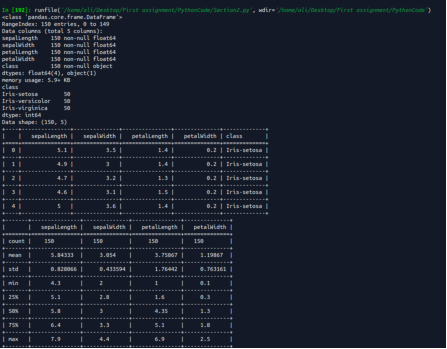
\includegraphics[width=15cm, height=17cm]{ss5}
\subsubsection{C)}
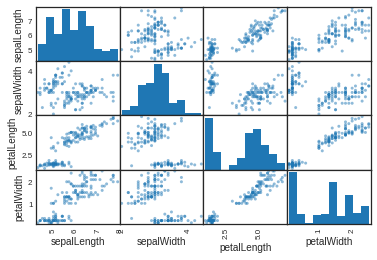
\includegraphics[width=6cm, height=6cm]{ScatterPlot}
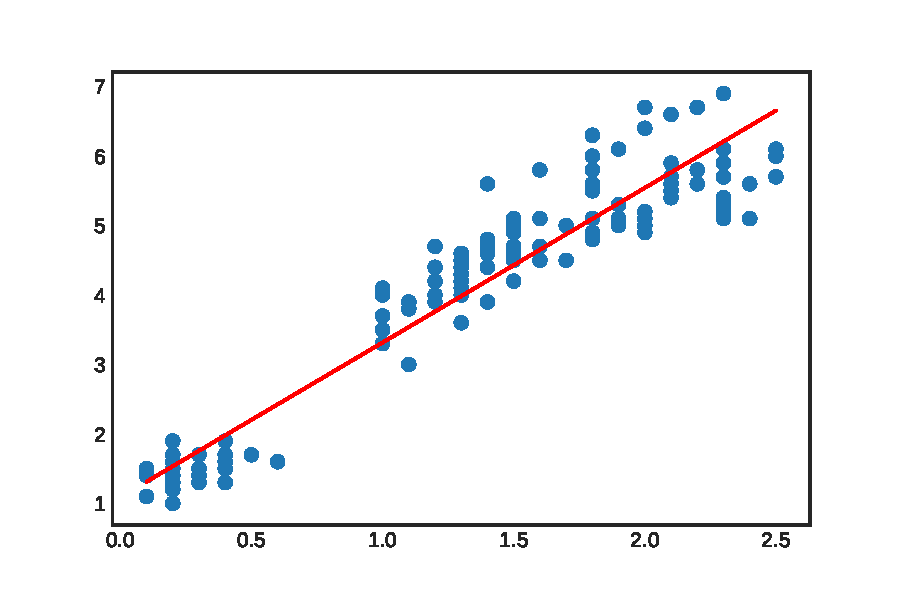
\includegraphics[width=8cm, height=6.5cm]{LR}\\\\
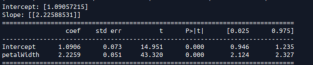
\includegraphics[width=15cm, height=3cm]{ss6}
\subsubsection{D)}\
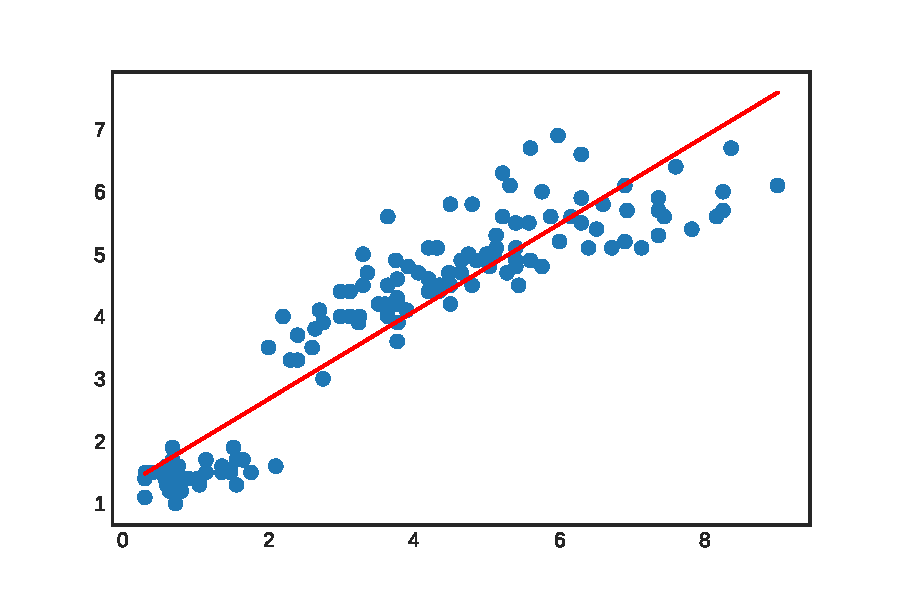
\includegraphics[width=8cm, height=6.5cm]{LR_mul}\\
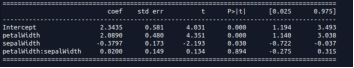
\includegraphics[width=15cm, height=3cm]{E}\\\\\\
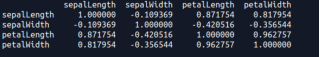
\includegraphics[width=15cm, height=3cm]{ss9}\\
The p-value of petalWidth*sepalWidth is 0.894 which is large so we conclude that feature petalWidth*sepalWidth cannot improve our model.\\\\
\href{https://github.com/zamaniali1995/Linear-Regressions-and-Linear-Models-using-the-Iris-Data}{Source Code}
\end{document}